\documentclass[epsfig,10pt,fullpage]{article}

\newcommand{\LabNum}{8}
\newcommand{\CommonDocsPath}{../../../../common/docs}
\input{\CommonDocsPath/preamble.tex}

\begin{document}

\centerline{\huge Computer Organization}
~\\
\centerline{\huge Laboratory Exercise \LabNum}
~\\
\centerline{\large Introduction to Graphics and Animation}
~\\

The purpose of this exercise is to learn how to display images and perform animation. 
We assume that you are using the {\it DE1-SoC Computer System with Nios~V},
which is described as part of the \texttt{Computer Organization} course on the website
{\href{https://www.fpgacademy.org/courses.html} {FPGAcademy.org}}.
A good approach is to first implement your C code for each part of this exercise by 
using the {\it CPUlator} simulator, and then to implement your solution in a hardware board,
if available.  If a hardware system other than the DE1-SoC Computer is being used, then 
some parts of this exercise may need to be modified to suit the features of your board. 

\section*{Background Information}
\addcontentsline{toc}{section}{Background Information}
The {\it DE1-SoC Computer with Nios~V} includes a video-out port with a VGA
controller that can be connected to a standard VGA monitor. The VGA controller supports
a screen resolution of 640 $\times$ 480. The image that is displayed by the VGA controller is
derived from two sources: a {\it pixel} buffer, and a {\it character} buffer. We will 
mainly focus on the pixel buffer in this exercise. 

\subsection*{Pixel Buffer}
\label{sec:pixel_buffer}
\addcontentsline{toc}{subsection}{Pixel Buffer}
The pixel buffer for the video-out port holds the data (color) for each pixel that is 
displayed by the VGA controller.  As illustrated in Figure \ref{fig:video_coord}, the
pixel buffer provides an image resolution of 
320 $\times$ 240 pixels, with the coordinate 0,0 being at the top-left corner of the image. 
Since the VGA controller supports the screen resolution of 640 $\times$ 480, each of the
pixel values in
the pixel buffer is replicated in both the {\it x} and {\it y} dimensions when it is being
displayed on the VGA screen.

\begin{figure}[h!]
   \begin{center}
       \includegraphics{figures/fig_video_coord.pdf}
   \end{center}
   \caption{Pixel buffer coordinates.}
	\label{fig:video_coord}
\end{figure}


Figure \ref{fig:pixels}$a$ shows that each pixel color is represented as a 16-bit halfword, 
with five bits for the blue and red 
components, and six bits for green.  As depicted in part $b$ of Figure \ref{fig:pixels}, 
pixels are addressed in the pixel buffer by 
using the combination of a {\it base} address and an {\it x,y} offset.  In the computer systems
the default address of the pixel buffer is {\sf 0x08000000},
which corresponds to the starting address of the FPGA on-chip memory.
Using this scheme, the pixel at location 0,0 has the address {\sf 0x08000000}, 
the pixel 1,0 has the address {\it base} $+$ (00000000~000000001~0)$_2$ = {\sf 0x08000002}, 
the pixel 0,1 has the address {\it base} $+$ (00000001~000000000~0)$_2$ = {\sf 0x08000400}, and 
the pixel at location 319,239 has the address {\it base} $+$ (11101111 100111111 0)$_2$ = 
{\sf 0x0803BE7E}. 

\begin{figure}[h!]
   \begin{center}
       \includegraphics{figures/fig_pixels.pdf}
   \end{center}
   \caption{Pixel values and addresses.}
	\label{fig:pixels}
\end{figure}

You can create an image by writing color values into the pixel addresses as described
above. A dedicated {\it pixel buffer controller} reads this pixel data from the memory and 
sends it to the VGA display.  The controller reads the pixel data in sequential order, 
starting with the pixel data corresponding to the upper-left corner of the VGA screen and 
proceeding to read the whole buffer until it reaches the data for the lower-right corner. This 
process is then repeated, continuously.  You can modify the pixel data at any time, by writing 
to the pixel addresses. Writes to the pixel buffer are automatically interleaved in the 
hardware with the read operations that are performed by the pixel buffer controller. 

~\\
It is also possible to prepare a new image for the VGA display without changing the content 
of the pixel buffer, by using the concept of {\it double-buffering}.  In this scheme two 
pixel buffers are involved, called the {\it front} and {\it back} buffers, as described below.

\subsection*{Double Buffering}
\label{sec:double_buffer}
\addcontentsline{toc}{subsection}{Double Buffering}
As mentioned above, a pixel buffer controller reads data out of the pixel buffer so that it 
can be displayed on the VGA screen. This pixel buffer controller 
includes a programming interface in the form of a set of registers, as
illustrated in Figure~\ref{fig:pixel_ctrl}.
The {\it Buffer} and {\it Backbuffer} registers each store the starting address of a pixel buffer.
The Buffer register holds the address of the pixel buffer that is displayed on the VGA screen.
As mentioned above, in the default configuration this Buffer register is set to the address {\sf 0x08000000}.
The default value of the Backbuffer register is also {\sf 0x08000000}, which means that there is only one pixel buffer.
Software can modify the address stored in the Backbuffer register, thereby creating a second pixel buffer.
An image can be drawn into this second buffer by writing to its pixel addresses.
This image is not displayed on the VGA monitor until a pixel buffer {\it swap} is performed, as explained below.

~\\
A pixel buffer swap is caused by writing the value 1 to the Buffer register. This write
operation does not directly modify the content of the Buffer register, but instead causes
the contents of the Buffer and Backbuffer registers to be swapped. The swap operation does
not happen right away; it occurs at the end of a VGA screen-drawing cycle, after the last 
pixel in the bottom-right corner has been displayed. This time instance is referred to as
the {\it vertical synchronization} time, and occurs every 1/60 seconds. Software can poll the
value of the $S$ bit in the {\it Status} register to see when the vertical synchronization has happened.
Writing the value 1 into the Buffer register causes $S$ to be set to 1. Then, when the swap of
the Buffer and Backbuffer registers has been completed $S$ is reset back to 0. The {\it Status}
register, shown in Figure~\ref{fig:pixel_ctrl}, contains additional bits of information,
but these bits are not needed for this exercise.  Also, the programming interface includes
a {\it Resolution} register, shown in the figure, that contains the {\it X} and {\it Y}
dimensions of the pixel buffer(s).  

\begin{figure}[h!]
   \begin{center}
       \includegraphics{figures/fig_video_port.pdf}
   \end{center}
   \caption{Pixel buffer controller registers.}
	\label{fig:pixel_ctrl}
\end{figure}

~\\
In a typical application the pixel buffer controller is used as follows. While the image
contained in the pixel buffer that is pointed to by the Buffer register is being displayed, 
a new image is drawn into the pixel buffer pointed to by the Backbuffer register. When this new
image is ready to be displayed, a pixel buffer swap is performed. Then, the pixel buffer 
that is now pointed to by the Backbuffer register, which was already displayed, is cleared and 
the next new image is drawn. In this way, the next image to be displayed is always drawn into
the ``back'' pixel buffer, and the ``front'' and ``back'' buffer pointers are swapped when 
the new image is ready to be displayed. Each time a swap is performed software has to 
synchronize with the VGA controller by waiting until the $S$ bit in the Status register becomes 0.

\section*{Part I}
\addcontentsline{toc}{section}{Part I}
In this part you will learn how to implement a simple line-drawing algorithm.

~\\
Drawing a line on a screen requires coloring pixels between two points $(x_1,y_1)$ and 
$(x_2,y_2)$, such that the pixels represent the desired line as closely as possible. Consider 
the example in Figure~\ref{fig:line_drawing}, where we want to draw a line between 
points $(1,1)$ and $(12,5)$. The boxes in the figure represent the location and size of pixels
on the screen. As indicated in the figure, we cannot draw the line precisely---we can
only draw a shape that is similar to the line by coloring the pixels that fall closest to 
the line's ideal location on the screen.

\begin{figure}[h!]
   \begin{center}
       \includegraphics{figures/fig_line_drawing}
   \end{center}
   \caption{Drawing a line between points $(1,1)$ and $(12,5)$.}
	\label{fig:line_drawing}
\end{figure}

We can use algebra to determine which pixels to color. This is done by using the end points and 
the slope of the line. The slope of our example line is $slope = (y_2 - y_1)/(x_2 - x_1) = 4/11$. 
Starting at point $(1,1)$ we move along the $x$ axis and compute the $y$ coordinate for the 
line as follows:

\begin{eqnarray*}
y = y_1 + slope \times (x - x_1)
\end{eqnarray*}

Thus, for column $x = 2$, the $y$ location of the pixel is
$1 + \frac{4}{11} \times (2-1) = 1 \frac{4}{11}$. 
Since pixel locations are defined by integer values we round the $y$ coordinate to the nearest 
integer, and determine that in column $x = 2$ we should color the pixel at $y = 1$. For
column $x = 3$ we perform the calculation $y = 1 + \frac{4}{11} \times (3-1) = 1
\frac{8}{11}$, and round the result to $y = 2$.  Similarly, we perform such computations 
for each column between $x_1$ and $x_2$.

~\\
The approach of moving along the $x$ axis has drawbacks when a line is steep. A steep line
spans more rows than it does columns, and hence has a slope with absolute value greater than 
1.  In this case our calculations will not produce a smooth-looking line.  Also, in the case
of a vertical line we cannot use the slope to make a calculation.  To address this 
problem, we can alter the algorithm to move along the $y$ axis when a line is steep. With 
this change, we can implement a line-drawing algorithm known as {\it Bresenham's algorithm}.
Pseudo-code for this algorithm is given in Figure~\ref{fig:line_algorithm}. The first 15
lines of code set up the variables needed by the algorithm. 
Then, in lines 17 to 22 the algorithm increments the {\it x} variable 1 step at a time
and computes the {\it y} value. The {\it y} value is incremented when needed to stay as
close to the ideal location of the line as possible. Bresenham's algorithm calculates an
{\it error} variable to decide whether or not to increment each {\it y} value. The version
of the algorithm shown in Figure~\ref{fig:line_algorithm} uses only integers to perform
all calculations.  To understand how this algorithm works, you can read about Bresenham's
algorithm in a textbook or by searching for it on the internet.

\begin{figure}[th]
	\centering
		\begin{lstlisting}[numbers=left, stepnumber=1, xleftmargin=1cm]
  draw_line(x0, x1, y0, y1)
		
		boolean is_steep = abs(y1 - y0) > abs(x1 - x0)
		if is_steep then
			swap(x0, y0)
			swap(x1, y1)
		if x0 > x1 then
			swap(x0, x1)
			swap(y0, y1)
			
		int deltax = x1 - x0
		int deltay = abs(y1 - y0)
		int error = -(deltax / 2)
		int y = y0
		if y0 < y1 then y_step = 1 else y_step = -1
		
		for x from x0 to x1
			if is_steep then draw_pixel(y, x) else draw_pixel(x, y)
			error = error + deltay
			if error >= 0 then
				y = y + y_step
				error = error - deltax
			
\end{lstlisting}
	\caption{Pseudo-code for a line-drawing algorithm.}
	\label{fig:line_algorithm}
\end{figure}

Perform the following:

\begin{enumerate}

\item Write a C-language program that implements Bresenham's line-drawing algorithm,
and uses this algorithm to draw a few lines on the screen.  An example of a suitable main 
program is given in Figure~\ref{fig:main1}. The code first determines the address of the 
pixel buffer by reading from the pixel buffer controller, and stores this address into the
global variable {\it pixel\_buffer\_start}. The main program clears the screen, and then 
draws four lines.  You have to write the {\it clear\_screen} function, which sets all
pixels to the color black (0), and the {\it draw\_line} function that implements
Bresenham's algorithm.  An example of a function that uses the global variable 
{\it pixel\_buffer\_start} is shown at the end of Figure~\ref{fig:main1}. The function 
{\it plot\_pixel ()} sets the pixel at location {\it x}, {\it y} to the color {\it line\_color}. 

\item Compile and test your solution. If you are using the {\it CPUlator}, then your VGA output
will be shown in the simulated \texttt{VGA pixel buffer} window pane. If you are using an
actual DE1-SoC board, then connect a VGA monitor to the board to see the video output.
\end{enumerate}

\begin{figure}[th]
\centering
\lstinputlisting[language=C]{../design_files/part1.c}
\caption{Main program for Part I.}
\label{fig:main1}
\end{figure}

\newpage
\section*{Part II}
\addcontentsline{toc}{section}{Part II}
Animation is an exciting part of computer graphics. Moving a displayed object is an illusion 
created by showing this same object at different locations on the screen. A simple way to
``move'' an object is to first draw the object at one position, and then after a short time erase 
the object and draw it again at another nearby position.

~\\
To realize animation it is necessary to move objects at regular time intervals. The VGA controller 
in the DE1-SoC Computer redraw the screen every $1/60^{th}$ of a second. Since the image on 
the screen cannot change more often than that, it is reasonable to control an animation
using this unit of time.

~\\
To ensure that you change the image only once every $1/60^{th}$ of a second, use the 
pixel buffer controller to synchronize with the vertical synchronization cycle of the VGA 
controller. As we discussed in the background section of this exercise, synchronizing with the 
VGA controller can be accomplished by writing the value 1 into the {\it Buffer} register in the 
pixel buffer controller, and then waiting until bit $S$ of the {\it Status} register becomes 
equal to 0. For this part of the exercise you do not need to use a back buffer, so ensure
that the {\it Buffer} and {\it Backbuffer} addresses in the pixel buffer controller are the 
same. In this approach, a pixel buffer ``swap'' can be used as a way of synchronizing with 
the VGA controller via the {\it S} bit in the {\it Status} register.

~\\
Perform the following:

\begin{enumerate}

\item Write a C-language program that moves a horizontal line up and down on the screen and 
``bounces'' the line off the top and bottom edges of the display. Your program should first 
clear the screen and draw the line at a starting row on the screen. Then, in an endless
loop you should erase the line (by drawing the line using black), and redraw it one row
above or below the last one.  When the line reaches the top, or bottom, of the screen 
it should start moving in the opposite direction.

\item Compile and test your solution. Notice how long it takes for the 
horizontal line to move through the 240 lines of the VGA display. On an actual DE1-SoC
board, it should take $240 \times 1/60 = 4$ seconds. If using the {\it CPUlator}
simulator, then the movement of the line up and down on the simulated screen will likely
be somewhat slower than in the real hardware.
\end{enumerate}

\section*{Part III}
\addcontentsline{toc}{section}{Part III}
Having gained the basic knowledge about displaying images and animations, you can now create 
a more interesting animation.

~\\
You are to create an animation of several small square boxes on the screen. These boxes 
should appear to be moving continuously and ``bouncing'' off the edges of the screen. Each
box should be filled with a color and the
boxes should be connected with lines to form a chain. An illustration of the animation 
is given in Figure~\ref{fig:animation_example}. Part $a$ of the figure shows one position
of the boxes with arrows that indicate the directions of movement, and 
Figure~\ref{fig:animation_example}$b$ shows a subsequent position of the boxes. 
In each step of your animation each of the boxes should appear to ``move'' on a diagonal 
line: up/left, up/right, down/left, or down/right. Move the boxes one
row and one column at a time on the VGA screen.

\begin{figure}[h!]
   \begin{center}
       \includegraphics[scale = 0.5]{figures/fig_animation_example.pdf}
   \end{center}
   \caption{Two instants of the animation.}
	\label{fig:animation_example}
\end{figure}

To make the animation look slightly different each time you run it, use the C library function 
{\it rand ()} to help calculate initial positions for each of the boxes, and to determine 
their directions of movement. To add variety to your animations, you might randomly
have some boxes moving on diagonals, some moving vertically or horizontally, and some in fixed
positions.

~\\
Perform the following:

\begin{enumerate}

\item Write a C program to implement your animation. Use both a front and back buffer 
in your program, so that you can avoid making changes to the image while it is being displayed 
by the pixel buffer controller.  An example of a suitable main program (not all of the
code is shown) is given in Figure~\ref{fig:main3}. The code sets one pixel buffer to be 
in the FPGA on-chip memory (which is its default location), and
declares an array in the SDRAM memory to use as the location of the other pixel buffer
(the FPGA on-chip memory is not large enough to hold two pixel buffers). 
In each iteration of
the while loop the code clears the entire screen, draws the boxes and lines, and then 
updates the locations of boxes. At the bottom of the while loop the code calls the
function {\it wait\_for\_vsync ()}, which synchronizes with the VGA controller and swaps the 
front and back pixel buffer pointers.

\item Compile, debug, and test your code.

\item Experiment with your code by modifying it to use just a single pixel buffer (simply
change the address of the back buffer to be the same as the front buffer). Observe what you 
see on the VGA screen as a result of this change.
\end{enumerate}

\begin{figure}[H]
\centering
\lstinputlisting[language=C]{../design_files/part3.c}
\caption{Main program for Part III.}
\label{fig:main3}
\end{figure}

Instead of clearing the whole screen in each step of the animation, you may want to keep
track of where boxes and lines are drawn and then clear only the corresponding pixels (by
drawing in black) rather than the whole screen. This optimization makes your animation
more efficient and may make the boxes and lines move more smoothly.
\newpage
\section*{Part IV}
\addcontentsline{toc}{section}{Part IV}
For this part of the exercise you are to enhance the animation from Part~III so that
during the animation the following changes can take place:

\begin{enumerate}
\item
The speed of movement of the boxes can be increased or decreased
\item
The number of boxes can be increased or decreased
\item
The lines between boxes can be drawn or not drawn
\end{enumerate}

In Part III the speed of animation was set by the 1/60 seconds VGA vertical synchronization time.
One way to structure the program such that the animation timing can be changed is to use 
a timer. In this scheme you would wait for the timer, using polled-I/O before drawing
each frame of the animation.  Reducing the
timer frequency would cause the animation to appear to move more slowly. Increasing the
timer frequency would make the animation move more quickly, with the maximum speed being limited
by the 1/60 seconds VGA synchronization time, as it was in Part III.  To cause the animation 
to appear to move more quickly than in Part III, you have to increase the amount that the 
boxes are moved for each animation frame.

~\\
Perform the following:

\begin{enumerate}

\item Implement the speed control discussed above for the animation. The speed of animation 
should approximately double when you press pushbutton {\it KEY}$_0$, and it should reduce by 
the same amount when you press {\it KEY}$_1$. Pressing {\it KEY}$_2$ should add a box to the
animation, up to some maximum of your choosing. Pressing {\it KEY}$_3$ should remove a
box. Finally, when any of the {\it SW} slider switches is set to the 1 position the lines 
between boxes should not be drawn; only when all switches are set to the 0 position should 
the lines appear.

\item Compile, debug, and test your code. 

\item Add any other animation features that you may find interesting. As an example, you
could make use of the character buffer in the DE1-SoC Computer to display text with your
animation. You could show a frame counter that indicates how many frames have been
displayed as the animation proceeds. The character buffer is described in the
documentation for the {\it DE1-SoC Computer with Nios~V}. 
\end{enumerate}


\input{\CommonDocsPath/copyright.tex}
\end{document}
